\documentclass[12pt]{report} 

% PACKAGES 
\usepackage[dutch]{babel}
\usepackage[utf8]{inputenc}
\usepackage{color}
\usepackage{amsmath} % Matrices
\usepackage{amsfonts}
\usepackage{booktabs}
\usepackage{xcolor}
\usepackage{sectsty}
\usepackage{graphicx}
\usepackage{lipsum}

\graphicspath{{img/}}

\newcommand{\answercolor}{teal}


\partfont{\color{brown}}
\chapterfont{\color{teal}}
\sectionfont{\color{cyan}}

% DOCUMENT INFORMATION
\title{Wiskunde A}
\author{Bert De Saffel}
\date{2017-2018}


% CUSTOM COMMANDS
\newcommand{\todo}[1] {
\color{red}\textunderscore{\textit{TODO: #1}}
}

\newcommand{\important}[1] {\textbf{\color{orange}#1}}
\newcommand{\mathimportant}[2] {\textbf{\color{#2}$#1$}}

% DOCUMENT
\begin{document}
\maketitle
\tableofcontents

\part{Theorie}
\chapter{Complexe Getallen}
\section{Inleiding}
\begin{itemize}
 \item $\mathbb{N}$ = Natuurlijke getallen: \{0, 1, 2, 3, ...\}
 \item $\mathbb{Z}$ = Gehele getallen: \{..., -2, -1, 0, 1, 2, ...\}
 \item $\mathbb{Q}$ = Rationale getallen: \{$\frac{1}{3}$, $-\frac{1}{4}$, $\frac{7}{2}$, ... \}
 \item $\mathbb{R}$ = Reële getallen: \{ $\sqrt{2}$ , $\pi$ \}
 \item $\mathbb{C}$ = Complexe getallen: $j^2 = -1$, $j = $ imaginaire eenheid
\end{itemize}

  $z = \mathimportant{a}{orange} + \mathimportant{b}{orange}j$ met $z \in \mathbb{C}$, $a \in \mathbb{R}, b \in \mathbb{R}$ en $j = \sqrt{-1}$
  \newline
  $Re(z) = a$
  \newline
  $Im(z) = b$

\section{Eigenschappen}
$\mathimportant{z_1}{orange} = a + bj$
\newline
$\mathimportant{z_2}{red} = c + dj$
 
\begin{itemize}
 \item Som: $\mathimportant{z_1}{orange} + \mathimportant{z_2}{red}
\newline
= \mathimportant{a + bj}{orange} + \mathimportant{c + dj}{red} 
\newline
= \mathimportant{a}{orange} + \mathimportant{c}{red} + (\mathimportant{b}{orange} + \mathimportant{d}{red})j$ 
  \item Product: $\mathimportant{z_1}{orange} \times \mathimportant{z_2}{red}$ 
\newline
  = $\mathimportant{(a + bj)}{orange} \times \mathimportant{(c + dj)}{red}$
\newline
  = $\mathimportant{a}{orange}\mathimportant{c}{red} + \mathimportant{a}{orange}\mathimportant{d}{red}j + \mathimportant{b}{orange}\mathimportant{c}{red}j + \mathimportant{b}{orange}\mathimportant{d}{red}j^2$
\newline
  = $\mathimportant{a}{orange}\mathimportant{c}{red} - \mathimportant{b}{orange}\mathimportant{d}{red} + (\mathimportant{a}{orange}\mathimportant{d}{red} + \mathimportant{b}{orange}\mathimportant{c}{red})j$
  \item Complex toegevoegde $\rightarrow$  $\overline{z} = a - bj$
\end{itemize}

\subsection{Oefening}
$z_1 = 2 + 3j$
\newline
$z_2 = 1 + 2j$

\begin{itemize}
 \item Som: $z_1 + z_2 
 \newline
 = (2 + 3j) + (1 + 2j) 
 \newline
 = 2 + 1 + 3j + 2j 
 \newline
 = \mathimportant{3 + 5j}{\answercolor}$ 
 \item Product: $z_1 * z_2 
 \newline
 = (2 + 3j) \times (1 + 2j) 
  \newline
 = 2 * 1 + 2 * 2j + 3j * 1 + 3j * 2j 
  \newline
 = 2 + 4j + 3j + 6j^2 
  \newline
 = 2 + 7j -6
  \newline
 = \mathimportant{-4 + 7j}{\answercolor}$
 \item Complex toegevoegde: \newline
 $\overline{z_1} = 2 - 3j$
 \newline
 $\overline{z_2} = 1 - 2j$
\end{itemize}

\section{Voorstellingen van een complex getal}
\begin{enumerate}
 \item {Cartesische vorm [$z = a + bj$]}
 \item {Goniometrische vorm [$z = r(cos\theta + jsin\theta$]}
 \item {Exponentiële vorm [$z = re^{j\theta}$]}
\end{enumerate}
\subsection{Cartesische vorm}
$z = a + bj$ 
\newline
Complex vlak: 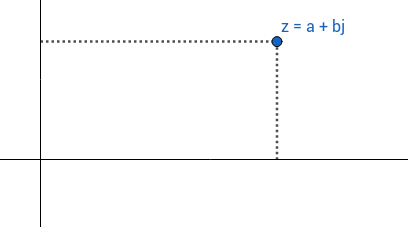
\includegraphics{cartesischevorm}



\end{document}
